\documentclass{article}
\usepackage{xeCJK}
\usepackage{ctex}
\usepackage{listings}
\usepackage{xcolor, xparse}
\usepackage{setspace}
\usepackage{graphicx}
\usepackage[left=2.50cm, right=2.50cm, top=2.50cm, bottom=2.50cm]{geometry}
\usepackage{makecell}
\usepackage[CJKbookmarks=true]{hyperref}

\definecolor{mygreen}{rgb}{0,0.6,0}
\definecolor{mygray}{rgb}{0.5,0.5,0.5}
\definecolor{mymauve}{rgb}{0.58,0,0.82}
\definecolor{darkblue}{rgb}{0, 0, 0.5}
\definecolor{cmdbg}{rgb}{0.8,0.8,0.8}
\definecolor{shadecolor}{rgb}{0.92,0.92,0.92}

\lstset{
    language    = c++,
    numbers     = left,
    rulesepcolor= \color{gray},
    breaklines=true,
    % backgroundcolor=\color{cmdbg},
    numberstyle={
        \small
        \color{gray}
    },
    commentstyle = \color{gray},
    keywordstyle={
        \color[RGB]{175,0,175}
        \bfseries
    },
    basicstyle={
        \small\ttfamily
    },
    breaklines=true,
    tabsize     = 4,
    frame       = single,%主题
    columns     = fullflexible,
    rulesepcolor = \color{red!20!green!20!blue!20}, %设置边框的颜色
    showstringspaces = false, %不显示代码字符串中间的空格标记
    escapeinside={\%*}{*)},
}

\lstdefinestyle{c++}{
    language    = c++,
    numbers     = left,
    rulesepcolor= \color{gray},
    breaklines=true,
    % backgroundcolor=\color{cmdbg},
    numberstyle={
        \small
        \color{gray}
    },
    commentstyle = \color{gray},
    keywordstyle={
        \color[RGB]{175,0,175}
        \bfseries
    },
    stringstyle={
        \color[RGB]{0,125,0}
        \bfseries
    },
    basicstyle={
        \small\ttfamily
    },
    breaklines=true,
    tabsize     = 4,
    frame       = single,%主题
    columns     = fullflexible,
    rulesepcolor = \color{red!20!green!20!blue!20}, %设置边框的颜色
    showstringspaces = false, %不显示代码字符串中间的空格标记
    escapeinside={\%*}{*)},
}

\lstdefinestyle{sql}{
    language    = sql,
    numbers     = left,
    rulesepcolor= \color{gray},
    breaklines=true,
    % backgroundcolor=\color{cmdbg},
    numberstyle={
        \small
        \color{gray}
    },
    commentstyle = \color{gray},
    keywordstyle={
        \color[RGB]{175,0,175}
        \bfseries
    },
    stringstyle={
        \color[RGB]{0,125,0}
        \bfseries
    },
    basicstyle={
        \small\ttfamily
    },
    breaklines=true,
    tabsize     = 4,
    frame       = single,%主题
    columns     = fullflexible,
    rulesepcolor = \color{red!20!green!20!blue!20}, %设置边框的颜色
    showstringspaces = false, %不显示代码字符串中间的空格标记
    escapeinside={\%*}{*)},
}




\begin{document}

\pagestyle{empty}
%生成封面
\begin{figure}
    \centering
    
\includegraphics[width=0.35\textwidth]{xdu.jpeg}
\end{figure}

\begin{spacing}{3.0}
    \centering
    \ \\
    \textbf{\Huge 编译实验实验报告}

    \Large 姓名: 施鹏飞 \\ 学号:18040100077 \\ 2021年6月30日
\end{spacing}
\newpage 

%生成目录
\setcounter{secnumdepth}{4} 
\setcounter{tocdepth}{4}  
\begin{spacing}{2.0}
    \tableofcontents
\end{spacing}
\newpage

\begin{spacing}{2}
\pagestyle{plain}
\setcounter{page}{1}
\section{实验内容}
    本次编译原理实验中,我们借助Lex/Yacc等分析工具,实现了一个较为简单的数据库系统。
    该数据库系统为磁盘数据库,将数据存储在本地,程序结束后数据不会消失。
    用户可以在终端输入SQL语句操作数据库,执行相应的SQL功能。
\section{实验环境}
    Ubuntu 20.04.2 LTS, flex 2.6.4, bison (GNU Bison) 3.5.1 以及C++开发环境。
\section{内容分析}
    首先,我们考虑希望实现的所有数据库功能及对应的SQL语句格式,罗列如下:

    \begin{table}[h]
    \centering
        \begin{tabular}{|c|c|}
        \hline \textbf{操作描述} & \textbf{SQL语句} \\
        \hline 创建数据库 & create database  \{数据库名\} \\
        \hline 删除数据库 & drop database  \{数据库名\}\\
        \hline 使用数据库 & use  \{数据库名\} \\
        \hline 显示所有数据库 & show databases \\
        \hline 创建表单 & create table \{列名 \space 列类型, ...\} \\
        \hline 删除表单 & delete table  \{表单名\} \\
        \hline 展示所有表单 & show tables \\
        \hline 展示某表单的属性 & desc  \{表单名\} \\
        \hline 插入 & insert into  \{表单名\} ... [where ...] \\
        \hline 查找 & select ... from  \{表单名, ...\} \\
        \hline 删除 & delete from  \{表单名\} [where ...] \\
        \hline 更新 & update  \{表单名\} set ... [where ...] \\
        \hline 删除表单 & drop table  \{表单名\} \\ 
        \hline 退出 & exit \\
        \hline 
        \end{tabular}
    \end{table}

    综合考虑后,我使用Lex生成文法记号,Yacc对语法进行分析,当识别出不同的命令时,再分不同的情况进行功能实现:

    \indent \space \space $\bullet$ 对于仅涉及到一、两个字符串的命令(如创建数据库、删除表单、退出等),Yacc直接将该字符串传给功能实现接口进行处理。

    \indent \space \space $\bullet$ 对于涉及到以列表形式给出指令(如创建数据表、插入元组、查找元组等)的情况时,Yacc在对语法树归结时,直接将SQL命令中的列表信息以\fcolorbox{black}{shadecolor}{\{内容所在的指针 + 内容有效字节\}}的格式一条条插入预先给出的全局链表中;
    当整条语句解析完成后,Yacc通知功能实现模块,功能实现模块访问该全局链表,按照预先商定好的顺序对其进行解析,进而完成SQL功能。

\section{具体实现}
    考虑到在本套系统中,Lex与其余部分的联系稍微弱一些,因而在本章节我们主要分\textbf{\textcolor{red}{三部分}}进行阐述。
    第一部分介绍Lex处理单词的方式,第二部分介绍数据库物理结构与逻辑结构,第三部分介绍Yacc对记号流的解析以及对应C++数据库操作接口的设计。
    \subsection{Lex词法分析}
        Lex负责解析输入的字符串,并将其转换为记号流传达给Yacc。
        \subsubsection{解析SQL关键字}
            用户可能输入SQL关键字,此时Lex不区分大小写的解析出他们,并输出对应的宏定义值。
            以几个SQL关键字为例,给出代码详细说明Lex如何处理关键字:

            \textbf{定义部分}
                \begin{spacing}{1.15}
                \lstinputlisting[style=c++, firstline = 16, lastline=20]{../src/a.l}
                \end{spacing}
            
            \textbf{识别规则部分} 
            
                全部大写的返回值为Yacc中预先宏定义的常量值。
                \begin{spacing}{1.15}
                \lstinputlisting[firstline = 41, lastline=45]{../src/a.l}
                \end{spacing}

        \subsubsection{解析自定义的字串}
            用户可能输入如下三种自定义的类型:

                \indent \indent $\bullet$ 整数(由0-9构成的数,允许前导0)

                \indent \indent $\bullet$ 字符串(在本实验中我们认为字符串必须以\textbf{双引号}为首尾,暂不与标准SQL对应)
                
                \indent \indent $\bullet$ 变量名(包含数字、52个大小写字母与下划线,且不以数字开头)。

            \textbf{定义部分}

            两个基本的类型\fcolorbox{black}{shadecolor}{charType}和\fcolorbox{black}{shadecolor}{digitType}分别表示可用的字符以及10个数码。
            \fcolorbox{black}{shadecolor}{integer}是由若干个基本数码组成的一个合法的允许前导0的整数。
            \fcolorbox{black}{shadecolor}{id}以一个字符起头,随后跟任意数量(可以为0)的数码或字符。
            \fcolorbox{black}{shadecolor}{string}以双引号为首尾,中间有任意数量(可以为0)的数码或字符。

            \textbf{a.l}
            \begin{spacing}{1.15}
            \lstinputlisting[firstline = 6, lastline=11]{../src/a.l}
            \end{spacing}

            \textbf{识别规则部分}   

                当识别到了这三种记号时,Lex将其以字符串指针的形式存储在yylval中以供Yacc使用。
                \textbf{特别地},整数类型也以字符串存储,解析的工作交给后人进行。

            \textbf{a.l}
            \begin{spacing}{1.15}
            \lstinputlisting[firstline = 70, lastline=82]{../src/a.l}
            \end{spacing}

        \subsection{解析标点符号}
            下面给出所用到的全部标点信息。

            \textbf{a.l}
            \begin{spacing}{1.15}
            \lstinputlisting[firstline = 84, lastline=91]{../src/a.l}
            \end{spacing}



    \subsection{数据库系统的结构设计}
        \subsubsection{物理结构 \label{SecPhy}} 
            在本地磁盘上,数据库系统文件全部存放在\fcolorbox{black}{shadecolor}{DBMS/}文件夹下。
            在DBMS下有一份元数据\fcolorbox{black}{shadecolor}{.dbinfo},用于说明该数据库系统有哪些数据库。
            其中记载了明文形式的所有数据库名字,以供系统访问对应的次级文件夹。
            而在某一个数据库下,以\fcolorbox{black}{shadecolor}{Database1}为例,其所有的表单以及元数据全部存储在文件夹\fcolorbox{black}{shadecolor}{Database1/}下。
            在该文件夹下首先有一份元数据\fcolorbox{black}{shadecolor}{.tableinfo},用于说明该数据库下有哪些表单。其中记载了明文形式的所有表单名,以供系统进一步访问表单文件。
            每一份表单文件的文件名即为表单名,在其内部,数据按照如下的字节顺序排列:\\
                \indent \space \space $\bullet$ 前32位为一个$32$位整数$n$,表明该表单有多少个属性域。 \\
                \indent \space \space $\bullet$ 接下来跟$n$块数据代表属性域的详细属性。每一块数据前$32$位为为一个$32$位整数$l_i$,表示该属性域的名称长度,随后跟$l_i$字节的信息,代表该属性域的名称,
                再后跟2个32位整数,分别为该属性域的占用字节长度和属性类型。\\
                \indent \space \space $\bullet$ 然后32位为一个$32$位的整数$m$, 表明该表单有多少个元组。 \\
                \indent \space \space $\bullet$ 接下来跟$m$块数据代表表单的具体内容。每一块数据又分成$n$小块,这每一小块就代表了该元组在对应属性域上的分量。
                在每一小块中,首先给出$32$位的一个整数$k_i$,代表该元组在该属性上拥有$k_i$字节的信息,随后跟出$k_i$字节的数据,表明其具体的取值。
            

            尽管在上述具体阐述中,说明字节块的逻辑意义看起来可能较为费力,但是实际在对物理结构读写时只需要\fcolorbox{black}{shadecolor}{循环+字节读写}即可,比较方便。

            数据库系统的层次物理结构,如图\ref{FigStru}所示。
            
            \begin{figure}[h]
                \centering
                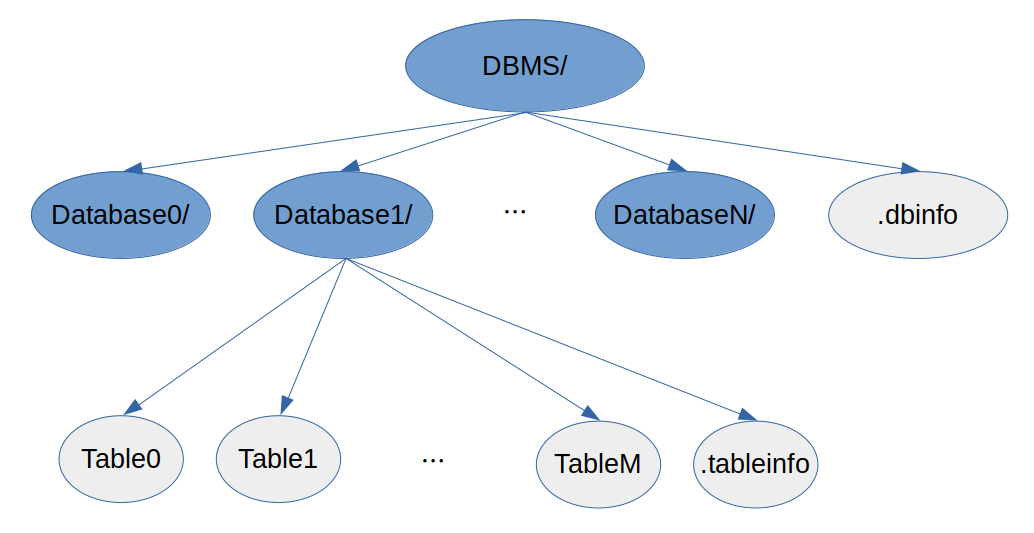
\includegraphics[width=0.7\textwidth]{structure.png}
                \caption{SQL系统文件层次结构} 
                \label{FigStru}                
            \end{figure}

        \subsubsection{逻辑结构}
            对应于\ref{SecPhy}给出的物理结构,我们对该数据库系统的逻辑存储结构进行说明。
            \paragraph{基本链表}
                本数据库系统使用自定义的链表结构,该链表的值域为\textbf{\textcolor{darkblue}{一个空指针与该空指针指向内容的有效字节长度}}。
                有了这样两条信息,我们就可以使用该链表存储任何信息,十分方便。
数据结构与函数接口如下所示。\\
                下面给出链表的数据接口与函数接口信息。\\
                \textbf{list.h}
                \begin{spacing}{1.15}
                \lstinputlisting[style=c++, firstline=15, lastline=33]{../src/list.h}
                \end{spacing}
            \paragraph{数据库系统结构}
                \fcolorbox{black}{shadecolor}{数据库系统}的结构较为简单,是一个链表元素为\fcolorbox{black}{shadecolor}{数据库}的链表。

                数据库系统提供如下的全局函数接口:创建数据库、使用数据库、删除数据库、显示所有的数据库、从本地读所有数据库、将所有数据库写入本地。
                
                数据结构与函数接口如下所示。\\
                \textbf{sql.h}
                \begin{spacing}{1.15}
                \lstinputlisting[style=c++, firstline=70, lastline=76]{../src/sql.h}
                \end{spacing}

            \paragraph{数据库结构}
                \fcolorbox{black}{shadecolor}{数据库}结构中有该数据库的名称,还有该数据库下所有表单形成的链表。

                对某个数据库而言,其提供如下的成员函数接口:查找某表单、显示所有表单、展示某表单的属性域、删除某表单、删除所有表单、从本地读数据库、将数据库写入本地。

                数据结构与函数接口如下所示。\\
                \textbf{sql.h}
                \begin{spacing}{1.15}
                \lstinputlisting[style=c++, firstline=52, lastline=64]{../src/sql.h}
                \end{spacing}
            \paragraph{表单结构}
            \fcolorbox{black}{shadecolor}{表单}结构中有该表单属于哪个数据库、该表单的名称、该表单拥有的属性数量、该表单的元组数量,以及所有属性构成的链表和所有元组构成的链表。
            
            \textbf{注意},在这里,一条元组本身就是一个链表,因而在该结构中,存储的元组链表其实是链表的链表。

            对于某个表单而言,其提供如下的成员函数接口:检查元组信息合法性(在where子句中用到,检查where子句约束的属性是否都确实是存在的一个合法属性)、
            展示表单所有属性域、从本地读表单、将表单写入本地。

            数据结构与函数接口如下所示。\\
            \textbf{sql.h}
            \begin{spacing}{1.15}
            \lstinputlisting[style=c++, firstline=38, lastline=50]{../src/sql.h}
            \end{spacing}

            \paragraph{属性域结构}
            \fcolorbox{black}{shadecolor}{属性域}结构记录了某属性的名称、占用的字节数以及其类型。
            属性域的类型是我们提前宏定义的整数类型,不同的整数代表不同的数据类型,目前暂时只支持\fcolorbox{black}{shadecolor}{INT}和\fcolorbox{black}{shadecolor}{CHAR()}。
            
            在属性域中有一个特别的值域\fcolorbox{black}{shadecolor}{selected},该属性仅在进行select操作时使用。
            当调用select语句时,首先检查所有的属性,如果select语句要求展示该属性则将\fcolorbox{black}{shadecolor}{selected}设置为真,不然则设置为假,最终在展示时我们就可以根据该值域的真假决定是否输出。

            数据结构与函数接口如下所示。\\
            \textbf{sql.h}
            \begin{spacing}{1.15}
            \lstinputlisting[style=c++, firstline=29, lastline=36]{../src/sql.h}
            \end{spacing}
            
            \paragraph{条件结构}
            \fcolorbox{black}{shadecolor}{条件}结构应用于where子句,用于记录某一个原子条件的信息。
            \textbf{注意}, 该结构体只能表示二元比较符,并且要求左操作数必须为数据属性,右操作数必须是属性值(如Age<20, Name < ``ZhangSan")。
            其内部有左操作数的指针及字节长度、右操作数的指针及字节长度、比较符的类型,比较符的类型预先进行了宏定义,是一个整数类型。

            数据结构如下所示。\\
            \textbf{sql.h}
            \begin{spacing}{1.15}
            \lstinputlisting[style=c++, firstline=23, lastline=27]{../src/sql.h}
            \end{spacing}
    \subsection{Yacc的语法分析并与接口的交互}
        考虑到Yacc在对语法树归结时会相应的进行语义翻译,二者联系十分密切,所以这里我们将两部分放在一起进行说明,以期能有更好的效果。
        在逐一说明各个功能的Yacc语法分析与C++接口使用方式之前,我们先给出Yacc用到的一些设置选项。

        \textbf{a.y}

        \begin{spacing}{1.15}
        \lstinputlisting[firstline=27, lastline=44]{../src/a.y}
        \end{spacing}

        结合Yacc文件的部分相关代码,我们做如下说明:

            \indent \indent $\bullet$ union联合体有三种可能的情况:字符串指针、32位整数、指针+字节数构成的结构体,在之后的程序中会根据不同的情况分配不同的数据类型。

            \indent \indent $\bullet$ \%token给出了可能Lex可能用到的宏定义,自动生成相应的存放在\fcolorbox{black}{shadecolor}{y.tab.h}中。

            \indent \indent $\bullet$ 由于版本不同,在本实验环境中我们使用\%type关键字来为文法中所有的终结符、非终结符分配类型。

            \indent \indent $\bullet$ 使用\%left指定左结合的优先级,解决多个逻辑表达式之间的组合问题。
        
        \subsubsection{总体语句框架}
            \fcolorbox{black}{shadecolor}{statements}由一条或多条的\fcolorbox{black}{shadecolor}{statement}组成。
            而每一个\fcolorbox{black}{shadecolor}{statement}则分别可能产生各种不同的非终结符,对应不同的功能;根据其返回值打印一定的提示信息。

            \textbf{a.y}
            \begin{spacing}{1.15}
            \lstinputlisting[firstline=48, lastline=97]{../src/a.y}
            \end{spacing}

        \subsubsection{创建数据库}
            为了创建数据库,只需要将数据库的名称作为当前语句的内容向上传,\fcolorbox{black}{shadecolor}{statement}调用\fcolorbox{black}{shadecolor}{create\_database}进行创建。

            \fcolorbox{black}{shadecolor}{create\_database}函数接受一个字符串及其字节数,首先检查当前数据库系统下是否存在一个同名的数据库,
            如果不存在,那么先在文件系统中创建一个对应的数据库文件夹,并在文件夹内创建一个数据表元数据(初始为空),
            再更新内存中的信息,创建一个新的数据库元素,将对应的值初始化后插入到数据库系统链表尾。至此全部操作完成。

            \textbf{a.y}
            \begin{spacing}{1.15}
            \lstinputlisting[firstline=99, lastline=100]{../src/a.y}
            \end{spacing}
            
        \subsubsection{使用数据库}
            使用数据库也类似地只需要将数据库的名称作为当前语句的内容向上传,\fcolorbox{black}{shadecolor}{statement}调用\fcolorbox{black}{shadecolor}{use\_database}进行选择。

            \fcolorbox{black}{shadecolor}{ues\_database}函数接受一个字符串及其字节数,检查该字符串对应的数据库是否存在,存在则操作成功。

            \textbf{a.y}
            \begin{spacing}{1.15}
            \lstinputlisting[firstline=102, lastline=103]{../src/a.y}
            \end{spacing}
        \subsubsection{显示所有数据库}
            显示数据库不需要任何用户自行输入的参数,只要归结成功\fcolorbox{black}{shadecolor}{statement}就调用\fcolorbox{black}{shadecolor}{show\_databases}展示所有的数据库。

            \fcolorbox{black}{shadecolor}{show\_databases}函数顺序遍历数据库系统链表中所有的数据表,并美观地将所有表名显示。

            \textbf{a.y}
            \begin{spacing}{1.15}
            \lstinputlisting[firstline=140, lastline=140]{../src/a.y}
            \end{spacing}
        \subsubsection{删除数据库}
            删除数据库也类似地将数据库名称向上传,statement调用\fcolorbox{black}{shadecolor}{statement}调用\fcolorbox{black}{shadecolor}{drop\_database}进行删除。

            \fcolorbox{black}{shadecolor}{drop\_database}函数接受一个字符串及其字节数,首先检查当前数据库系统下是否存在一个同名的数据库,
            如果存在,那么先在文件系统中删除对应的数据库文件夹,再更新内存中的信息,将该数据库对应的链表元素删去。至此全部操作完成。
            
            \textbf{a.y}
            \begin{spacing}{1.15}
            \lstinputlisting[firstline=258, lastline=259]{../src/a.y}
            \end{spacing}

        \subsubsection{创建表单}
            创建表单不仅需要表单名,还需要该表单各种属性的名称、类型、长度等信息,这些额外信息的数量未知,因而我们使用一个全局的\textbf{链表}来存储所有的这些信息。
            
            归结进行时首先肯定先读取到表单名时,将该字符串加入到链表,成为链表的第一个元素。

            接下来当归结到某一个属性域时,首先插入一个链表元素表示该属性的名称;
            接下来插入一个链表元素该元素的第一个字节表示该属性的类型,是一个提前约定好的整数,
            如果该类型是字符串数组,则该链表元素后面的所有字节则给出该数组的长度,以字符串形式给出,交由后人解析成整数。

            按照Yacc归结的顺序,可以保证该链表中所有的信息均是保持原有顺序的。

            当创建表单整条语句全部读取完成后,接口函数\fcolorbox{black}{shadecolor}{temp\_create\_table}就对该全局链表进行解析,创建相应的表单,这里就不予赘述了。

            \textbf{注意!}我们定义了一个全局的数据库指针\fcolorbox{black}{shadecolor}{current\_database}表明当前使用的数据库,在使用该创建表单功能前请先使用\fcolorbox{black}{shadecolor}{use}指令选定数据库,不然该函数将运行失败并给出相应的报错。
            在本报告之后也有一些SQL功能需要提前使用\fcolorbox{black}{shadecolor}{use}指令,之后便不再提及了,但是每一个之后对应的接口函数都对此做了错误处理,会产生相应的报错。

            \textbf{a.y}
            \begin{spacing}{1.15}
            \lstinputlisting[firstline=105, lastline=136]{../src/a.y}
            \end{spacing}
        \subsubsection{删除表单}
            删除表单跟之前的删除数据库很类似,上传表单名后statement使用\fcolorbox{black}{shadecolor}{drop\_table}指令。

            \textbf{a.y}
            \begin{spacing}{1.15}
            \lstinputlisting[firstline=255, lastline=256]{../src/a.y}
            \end{spacing}


        \subsubsection{显示所有表单}
            显示所有表单不需要额外的字符串参数,直接调用\fcolorbox{black}{shadecolor}{show\_tables}即可。

            \textbf{a.y}
            \begin{spacing}{1.15}
            \lstinputlisting[firstline=138, lastline=138]{../src/a.y}
            \end{spacing}
        \subsubsection{展示表单所有属性}
            展示表单上传表单名称,调用\fcolorbox{black}{shadecolor}{desc}成员函数即可。

            \textbf{a.y}
            \begin{spacing}{1.15}
            \lstinputlisting[firstline=142, lastline=142]{../src/a.y}
            \end{spacing}
        \subsubsection{插入元组}
            在insert功能下,我们支持两种插入模式。一种是不提供属性名,但是必须按顺序给全所有属性值;另一种提供属性名,相应地给出对应的属性值。

            \fcolorbox{black}{shadecolor}{insert\_values}对应解析出\fcolorbox{black}{shadecolor}{VALUE (属性值1,属性值2,...)}的结构。

            而\fcolorbox{black}{shadecolor}{insert\_method}则允许用户给出自定义的属性列,属性列之间用逗号分别,所有属性列用括号包围(哪怕是一个属性也需要括号)。

            根据插入模式的不同,信息在全局链表中的组成方式也不同。

            \indent \indent $\bullet$ 如果插入一条拥有全属性的元组,那么链表第一个元素记录了该表单的名称,用于函数索引出将要操作的表单;
            随后就给出所有属性域的内容以及长度直到结尾。接口函数会检查插入的属性值的数量是否与该表单拥有的属性属性匹配,但是暂时无法检测属性值的类型也匹配。
            
            \indent \indent $\bullet$ 如果插入一条只拥有部分属性的元组,那么链表第一个元素同样记录了该表单的名称,用于函数索引出将要操作的表单;
            随后跟一个有效字节长度为1、指针内容第一个字节为0的特征链表元素,表示即将开始属性名的插入。
            接下来跟着若干个链表元素,存储了将要插入元素拥有的属性名,以一个相同的特征0元素结束。
            当读取到第二个特征0元素后,就类似全属性元组结构一样,跟着所有对应的属性值直到文件结尾。

            接口函数 \fcolorbox{black}{shadecolor}{temp\_insert}解析该链表,并进行相应的插入工作,并会对一些常见错误进行汇报。当遇到一个不匹配的属性名后,该函数并不会报错,但也不会进行任何插入工作(此处没有与标准DBMS接轨,日后改进),那些没有初始值的属性值均被设置为空,展示时显示为\fcolorbox{black}{shadecolor}{(null)}.

            \textbf{a.y}
            \begin{spacing}{1.15}
            \lstinputlisting[firstline=144, lastline=188]{../src/a.y}
            \end{spacing}
        \subsubsection{查询元组}
            查询元组涉及到where条件子句,这里我们先对该类子句做一个说明。
            
            对于任意涉及到where字句的其余SQL语句,where都是可选的,因而在Yacc中 \fcolorbox{black}{shadecolor}{conditions}的解析也分为了有条件 \fcolorbox{black}{shadecolor}{with\_conditions}和无条件。

            那么有条件可以归约成若干条原子条件(即不包含逻辑与、逻辑或等,只有单独的一个逻辑表达式)的逻辑组合,正如\fcolorbox{black}{shadecolor}{with\_conditions}所示。

            在本实验中,暂只支持\fcolorbox{black}{shadecolor}{OR, AND}作为逻辑组合方式,\fcolorbox{black}{shadecolor}{<,=}作为逻辑比较符;
            尽管\fcolorbox{black}{shadecolor}{>, <=, >=}等其余运算符都能较快的通过\fcolorbox{black}{shadecolor}{<}来转换得到,但是在测试时仅采用了小于、等于这两个逻辑比较符,之后由于时间紧促,便没有来得及新加功能。

            在对条件进行归约的时候,我们使用\textbf{后缀表达式}解决优先级问题。使用后缀表达式不会产生优先级问题,使用一个栈线性地扫描就可以无歧义地完成解析工作。
            可以看到,在归约时,归约到\fcolorbox{black}{shadecolor}{value}时会向全局链表中加入数值/属性名,但归约到比较符时不进行任何操作,当整条逻辑比较语句全部读取完成后才将比较符加入到链表中。
            通过这样的归约方式,我们就可以获得所有条件的后缀表达式。

            因为字节长度的不同,所以接口函数可以通过分析字节长度来判断当前链表元素对应的是一个原子条件,还是一个逻辑组合符号。

            接口函数根据该全局链表解析条件,遍历查询的表单下的所有元组,如果当前元组符合所有的条件,则将该元组加入到一个候选元组链表中,该候选元组链表用于随后的输出。

            \textbf{需要注意}, 尽管这套DBMS的实现十分朴素,许多地方的时间复杂度、空间复杂度都没有仔细优化,但是这里由于涉及到了元组的复制,我们还是给出了一个较好的方法,以免出现复杂度爆炸:
                候选元组链表中不照搬复制原有的元组内容,而是存原有元组的指针信息。由于候选元组链表存的只是一个指针,那么其空间消耗至多也就是一个指针的大小加一个32位的整数,不会因为元组数据内容的巨大而消耗过多的时间空间。

            \textbf{a.y}
            \begin{spacing}{1.15}
            \lstinputlisting[firstline=190, lastline=216]{../src/a.y}
            \end{spacing}

            说明完了where子句对应的模块,剩余的部分就很简洁了。select语句要么使用\fcolorbox{black}{shadecolor}{*}要求显示所有的属性,要么给出需要的属性列表,以逗号分隔。本系统暂时只支持单表查询,不支持多表查询、子表查询等操作。

            在数据解析方面,由于有区分数据块归属的困难,我们再使用另一个全局的链表,与where子句使用的链表不同。这里使用的全局链表第一个元素给出表单的名称用于索引,随后给出所有希望查询的属性名;而where字句的链表专职处理逻辑语句的后缀表达式。

            接口函数\fcolorbox{black}{shadecolor}{temp\_select}会检查属性名是否正确,并对一些常见错误进行汇报,随后将美观地展示出所有元组的信息。

            \textbf{a.y}
            \begin{spacing}{1.15}
            \lstinputlisting[firstline=231, lastline=253]{../src/a.y}
            \end{spacing}
        \subsubsection{退出系统}
            读取到退出指令,系统先妥善地将内存数据库存储到本地,再安全地退出。

            \textbf{a.y}
            \begin{spacing}{1.15}
            \lstinputlisting[firstline=261, lastline=262]{../src/a.y}
            \end{spacing}


        \subsubsection{删除元组与更新元组}
            由于时间紧张等原因,delete和update操作并没有完成语义翻译,该系统暂时只能用Yacc解析出两种语句的结构,不能执行实际的操作,十分遗憾!

            \textbf{a.y delete}
            \begin{spacing}{1.15}
            \lstinputlisting[firstline=218, lastline=219]{../src/a.y}
            \end{spacing}

            \textbf{a.y update}
            \begin{spacing}{1.15}
            \lstinputlisting[firstline=221, lastline=229]{../src/a.y}
            \end{spacing}
    
\section{结果展示}
    使用如下的测试数据作为标准输入。

    \textbf{in}
    \begin{spacing}{1.15}
    \lstinputlisting[style=sql]{../src/in}
    \end{spacing}
    
    \ 

    测试结果如下所示,该系统能正确地执行上述语句。
    \begin{figure}[h]
    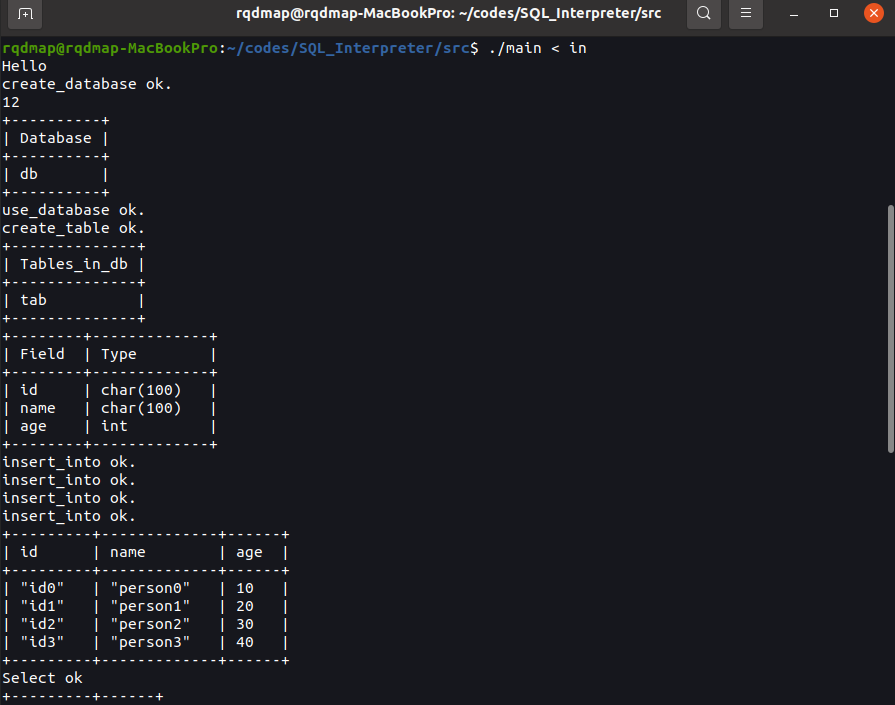
\includegraphics[width=1\textwidth]{out1.png}
    \end{figure}

    \begin{figure}[h]
    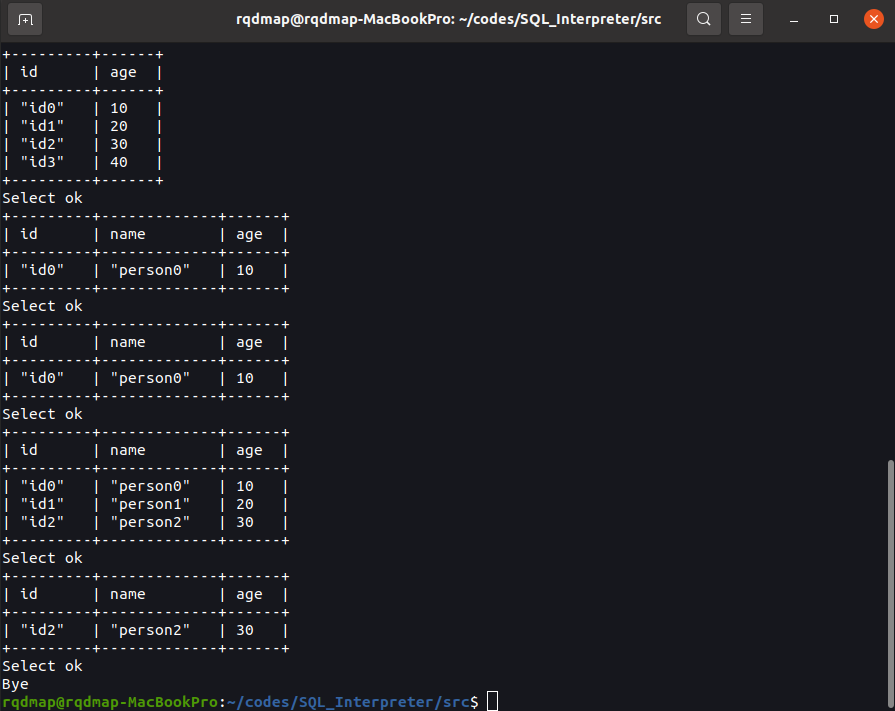
\includegraphics[width=1\textwidth]{out2.png}
    \end{figure}    

\section{局限与展望}
\begin{itemize}
    \item 该系统功能尚十分不完善,没有实现更新与删除操作,支持的数据类型、操作符、比较符不全面,不支持多表查询、子表查询,不支持主码、外码,不支持check语句,不支持数值表达式运算等。
    \item 该系统某些实现并没有与标准DBMS匹配,不能执行所有的标准SQL语句。
    \item 支持的条件类型十分单薄,不支持左值和右值的任意选择,可通过在条件结构体中添加数据类型进一步进行划分。
    \item 涉及到指定属性的函数操作并没有对该属性对应的数据类型进行合法性检查,默认用户遵循规范。
    \item 时空复杂度仍可以大力优化,并对代码和程序结构进一步美化。
\end{itemize}

\section{个人体会}
    本次实验我受益匪浅,熟悉了Lex/Yacc分析工具的使用,扎实了C++编程的功底,也提高了Latex书写文档的能力。
    半年来这是第三份千行代码以上的程序项目,从第一份RQD-FTP开始甚至不会写C++多文件编译、乱在h文件中写实现,到第二份二进制表示的高精度整数类,再到现在这份垃圾的DBMS全套系统,
    果然大工程使人提高,在神秘的方面提高了退役ACM选手的代码能力。正如小兵老师所说,这次实验项目令人难忘,自己实现DBMS十分有趣,但是实现出来的东西却差强人意。
    尽管有一千行左右但也就是我2天日夜肝出来的结果,日后如果有时间还希望进一步优化,能真正媲美一个标准的DBMS。\sout{当然,时空复杂度方面就不妄想与之比肩了,功能完备即心满意足了}


\section{程序清单}
\begin{table}[h]
    \begin{tabular}{|l|l|}
        \hline 
        程序名 & 描述 \\\hline
        MakeFile & \\\hline
        rqdmap.h & 个人编程惯用的一些宏定义 \\\hline
        list.h, list.cpp & 自定义链表结构接口及定义\\\hline
        a.l & Lex源文件 \\\hline
        lex.yy.c & Lex编译结果\\\hline
        a.y & Yacc文件 \\\hline
        y.tab.h, y.tab.c & Yacc编译结果\\\hline
        sql.h, sql.cpp & SQL函数接口及定义\\\hline
        main & 可执行程序,数据库系统\\\hline
        in & 测试数据 \\\hline
        init & bash脚本,初始化数据库\\\hline
        DBMS\ & 数据库本地文件 \\\hline

    \end{tabular}
\end{table}


\end{spacing}
\end{document}
